\documentclass[supercite]{Experimental_Report}

\title{~~~~~~新生实践课~~~~~~}
\author{刘伟灏}
\school{计算机科学与技术学院}
\classnum{2109}
\stunum{U202190077}
\instructor{陈加忠} % 李平、孙伟平、范晔斌、陈加忠
\date{2021年12月12日}

\usepackage{algorithm, multirow}
\usepackage{algpseudocode}
\usepackage{amsmath}
\usepackage{amsthm}
\usepackage{framed}
\usepackage{mathtools}
\usepackage{subcaption}
\usepackage{xltxtra} %提供了针对XeTeX的改进并且加入了XeTeX的LOGO, 自动调用xunicode宏包(提供Unicode字符宏)
\usepackage{bm}
\usepackage{tikz}
\usepackage{tikzscale}
\usepackage{pgfplots}
%\usepackage{enumerate}

\pgfplotsset{compat=1.16}

\newcommand{\cfig}[3]{
	\begin{figure}[htb]
		\centering
		\includegraphics[width=#2\textwidth]{images/#1.tikz}
		\caption{#3}
		\label{fig:#1}
	\end{figure}
}

\newcommand{\sfig}[3]{
	\begin{subfigure}[b]{#2\textwidth}
		\includegraphics[width=\textwidth]{images/#1.tikz}
		\caption{#3}
		\label{fig:#1}
	\end{subfigure}
}

\newcommand{\xfig}[3]{
	\begin{figure}[htb]
		\centering
		#3
		\caption{#2}
		\label{fig:#1}
	\end{figure}
}

\newcommand{\rfig}[1]{\autoref{fig:#1}}
\newcommand{\ralg}[1]{\autoref{alg:#1}}
\newcommand{\rthm}[1]{\autoref{thm:#1}}
\newcommand{\rlem}[1]{\autoref{lem:#1}}
\newcommand{\reqn}[1]{\autoref{eqn:#1}}
\newcommand{\rtbl}[1]{\autoref{tbl:#1}}

\algnewcommand\Null{\textsc{null }}
\algnewcommand\algorithmicinput{\textbf{Input:}}
\algnewcommand\Input{\item[\algorithmicinput]}
\algnewcommand\algorithmicoutput{\textbf{Output:}}
\algnewcommand\Output{\item[\algorithmicoutput]}
\algnewcommand\algorithmicbreak{\textbf{break}}
\algnewcommand\Break{\algorithmicbreak}
\algnewcommand\algorithmiccontinue{\textbf{continue}}
\algnewcommand\Continue{\algorithmiccontinue}
\algnewcommand{\LeftCom}[1]{\State $\triangleright$ #1}

\newtheorem{thm}{定理}[section]
\newtheorem{lem}{引理}[section]

\colorlet{shadecolor}{black!15}

\theoremstyle{definition}
\newtheorem{alg}{算法}[section]

\def\thmautorefname~#1\null{定理~#1~\null}
\def\lemautorefname~#1\null{引理~#1~\null}
\def\algautorefname~#1\null{算法~#1~\null}

\begin{document}
	
	\maketitle
	
	\clearpage
	
	\pagenumbering{Roman}
	
	\tableofcontents[level=2]
	\clearpage
	
	\pagenumbering{arabic}
	
	\section{网页整体框架}
	我的网页是为了讓人們更好地了解我的家鄉——澳門而創作的,其主要目的为体現出澳門獨有的中葡方化,在總体结构方面,我采用了总分分结构,即为一个主页和四个分页。其中,主页承担了引渡人們前往其他四个分页的重要职责,其不但特顯了主题中葡文化,更清晰地顯示了其他四个分页的内容,分别为“中葡文化歷史”“中葡人文”“中葡飲食”以及“多重国籍”。以下是网页的结构图。
	
	\begin{figure}[htb] % here top bottom
		\begin{center}
			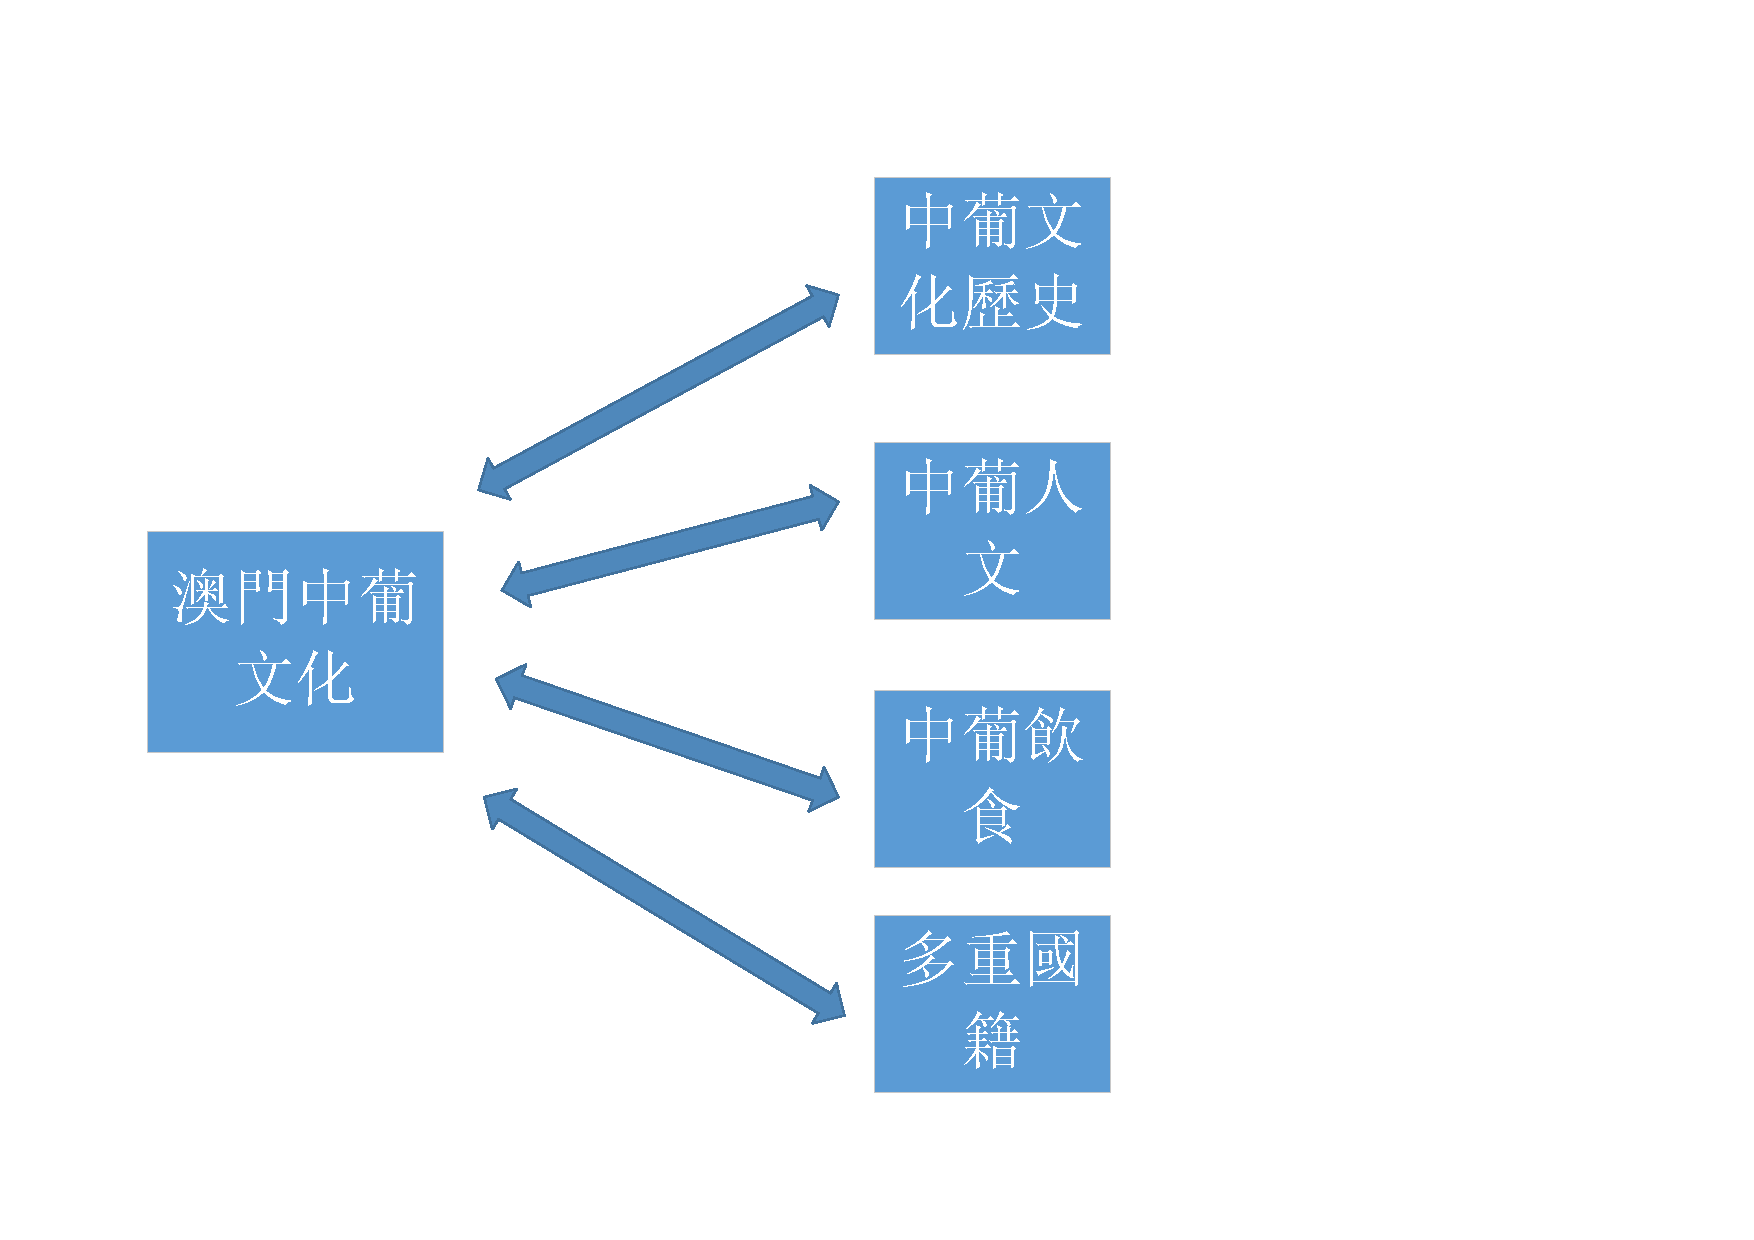
\includegraphics[scale=0.7]{images/1-1.pdf}
			\label{fig1-1}
		\end{center}
	\end{figure}
	其中主页不但能起到前往其他四个分页的功能,我更設置了回到寝室主页的功能。
	\newpage
	
	\section{主页设计}
	设计思路:我對网页的设计思路主要分为四大点,首先,网页的设计要紧扣我对网站的定义;其次,网页的設計要贴合到主题上;同時,首页设计尽量避免过于繁琐;最后,建站过程中要注意网站首页的加载速度。
	
	1.我对网站的定义:很多时候有些网站从视觉层面来看确实有着很高的水平,但就是网站在投入试运行后却并不能取得理想的效果,这种情况的发生绝大部分是因为在网站的整体设计下没有扣緊网站的定义定位。我認为在网站首页的设计当中,一定要更加注重对主题的突显,用多样的形式来表达网站的核心内容所在,但切莫让网页非常花哨却让人难以明白主题的方向在哪。
	
	2.网站的设计要贴合到主题上:关于首页的设计總会有不同的需求不同的内容展示,故对于首页的设计整体一定要做到贴好主题并独特精美,这一点不会难理解,在我的网页中,我采用澳门特色的中葡建筑,讓浏览网页的人能清晰了解此网页的功用。
	
	3.首页设计尽量避免过于繁琐:我在设计网站首页的时候,一开始投入了很大的精力与心思去把尽量多自己所认为好的相关内容素材都添加到网站的首页当中,结果卻令网页看起來雜亂不己,而操作起来也極为繁琐,故最后我采用了现在這種簡单的呈现手法,把其他四个分页的內容簡单明了地送到浏览者的手中,同时除去了一些不必要的元素,令操作亦不再繁琐。
	
	4.建站过程中要注意网站首页的加载速度:我認为网站页面的加载速度也極为重要,故在网站首页的设计时我特别注意在把相关内容的插入一定要保证好的加载速度,故我无有在首页放置图片、视频等内容,以免影响加载速度。
	以下是网页的截图:
	\begin{figure}[htb]
		\begin{center}
			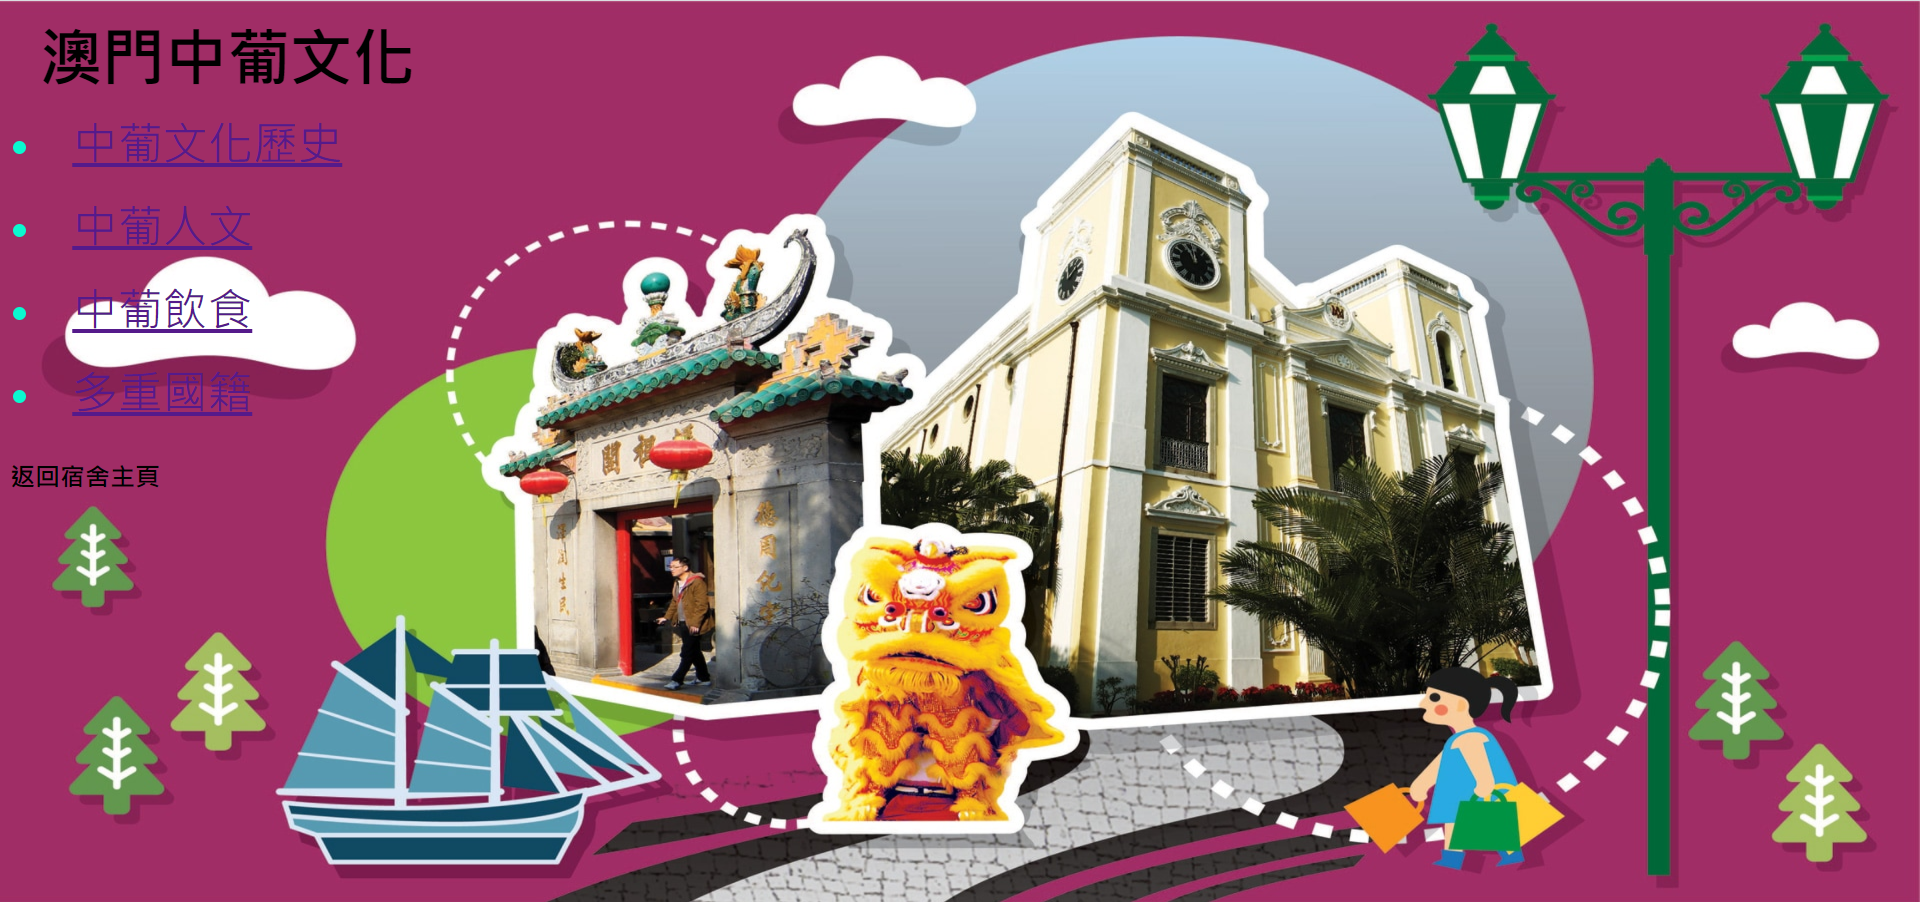
\includegraphics[scale=0.40]{images/2-1.jpg}
			\caption{主页举例}
			\label{fig2-1}
		\end{center}
	\end{figure}
	
	
	\newpage
	
	\section{分页面设计}
	
	
	\subsection{页面1 (中葡文化歷史)}
	在这个页面中,我簡单介绍了中葡文化的歷史,主要分为四点:
	
	首先,我介绍了澳门成为葡萄牙殖民地的重要过程,即《中葡和好通商條约》的簽定;
	
	然后,我著重地介绍了澳门回歸所经历的那十九年間發生的大事情,同時介绍了《中葡聯合聲明》這一重要條约;
	
	其次,描写出中葡文化所出现的原因,並利用圖片分享一些中葡文化所结合而成的特色産物,供浏览者觀看;
	
	最后,則是此分页的小结,讓浏览者了解這一文化出現的必然性,因其是经历了四百多年的演變,更受中、葡兩地不同文化彼此互相影响和吸收,最终而出現的澳门特色文化;
	
	以下是该网页的部分截图:
	\begin{figure}[htb] % here top bottom
		\begin{center}
			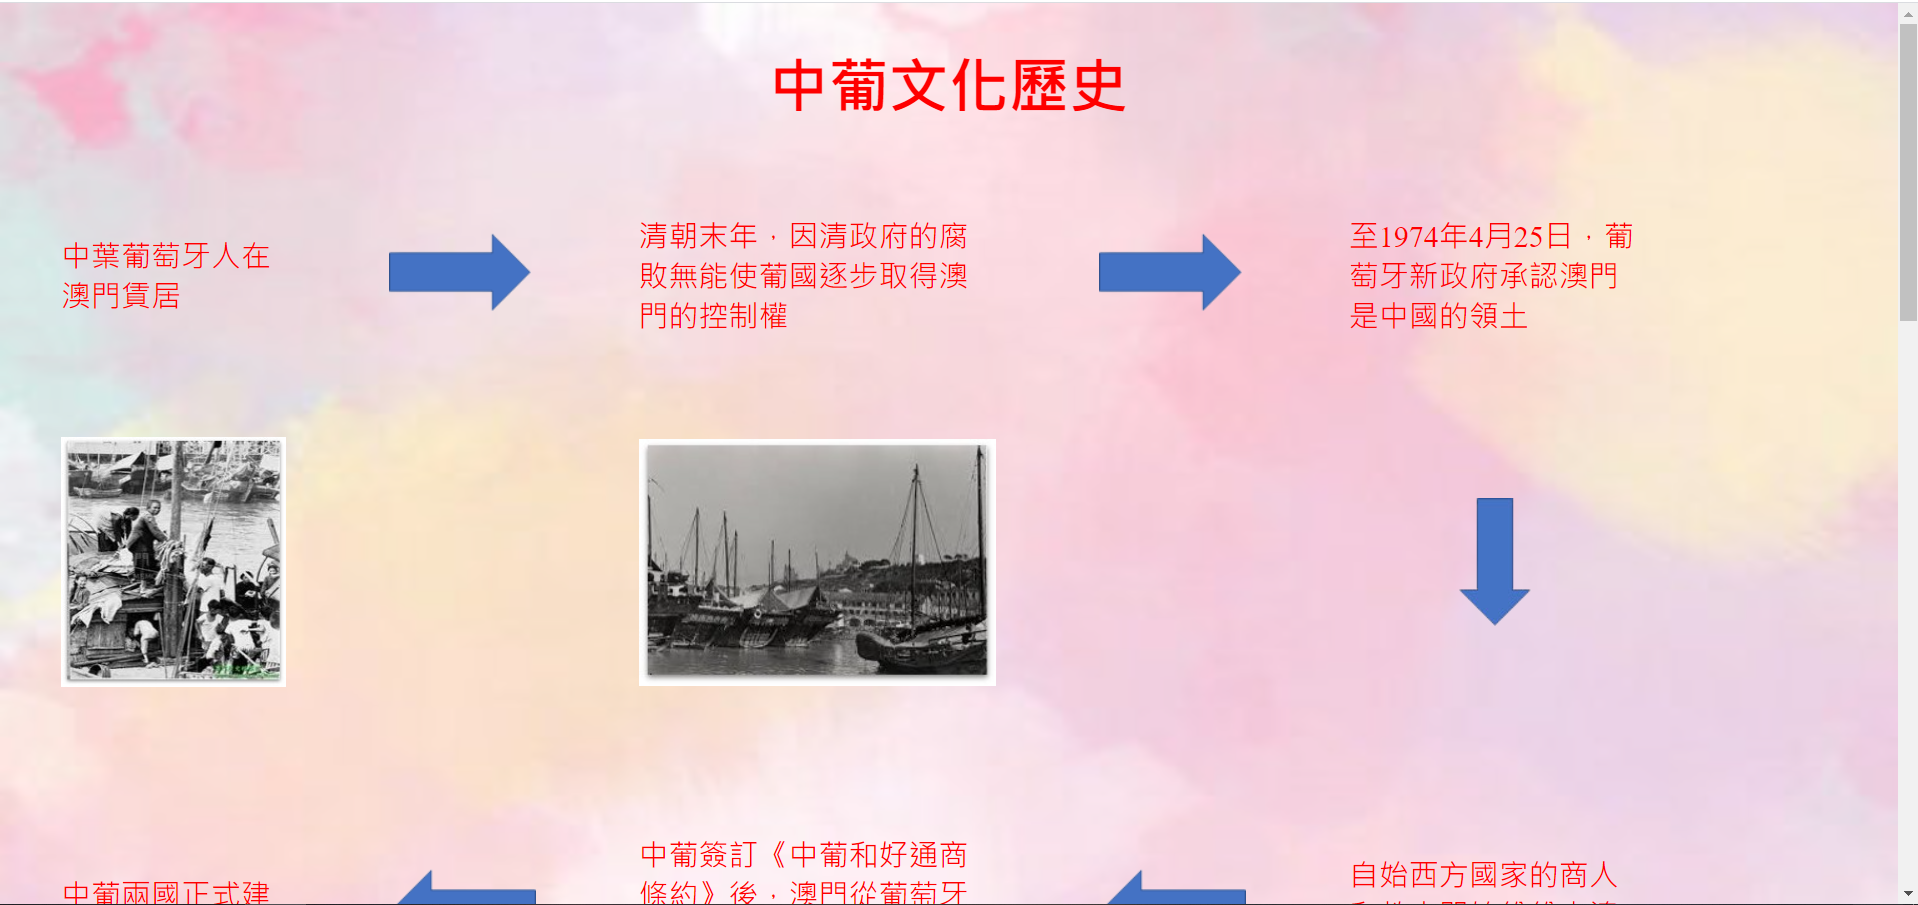
\includegraphics[scale=0.40]{images/3-1.jpg}
			\label{fig3-1}
			\caption{页面1 (中葡文化歷史)}
		\end{center}
	\end{figure}
	
	\newpage
	
	
	\subsection{页面2 (中葡人文)}
	此页面中介绍了中葡文化中的三大特点,分别为宗教、土生葡人和土生葡語。
	如何呈现這三大特点並不簡单,故我采用了图文并茂的方式,讓其表现得更清晰易懂。
	1.宗教:在宗教方面,我著重介绍了我們最大的宗教——天主教,分享了其進入澳门的过程和现今的發展情况,並以圖像形式呈现了其特色象徵——觀音蓮花苑。
	
	2.土生葡人:介绍了土生葡人的定义与其獨突之處,並表明了其現况。
	
	3.土生葡語:説明了其组成語言系统,介绍了土生葡語的别稱,和其歷史,讓浏览网页看了解到這项濒临的非物质文化遗产。
	
	以下是本网页的部分截图:
	
	
	\begin{figure}[htb]
		\begin{center}
			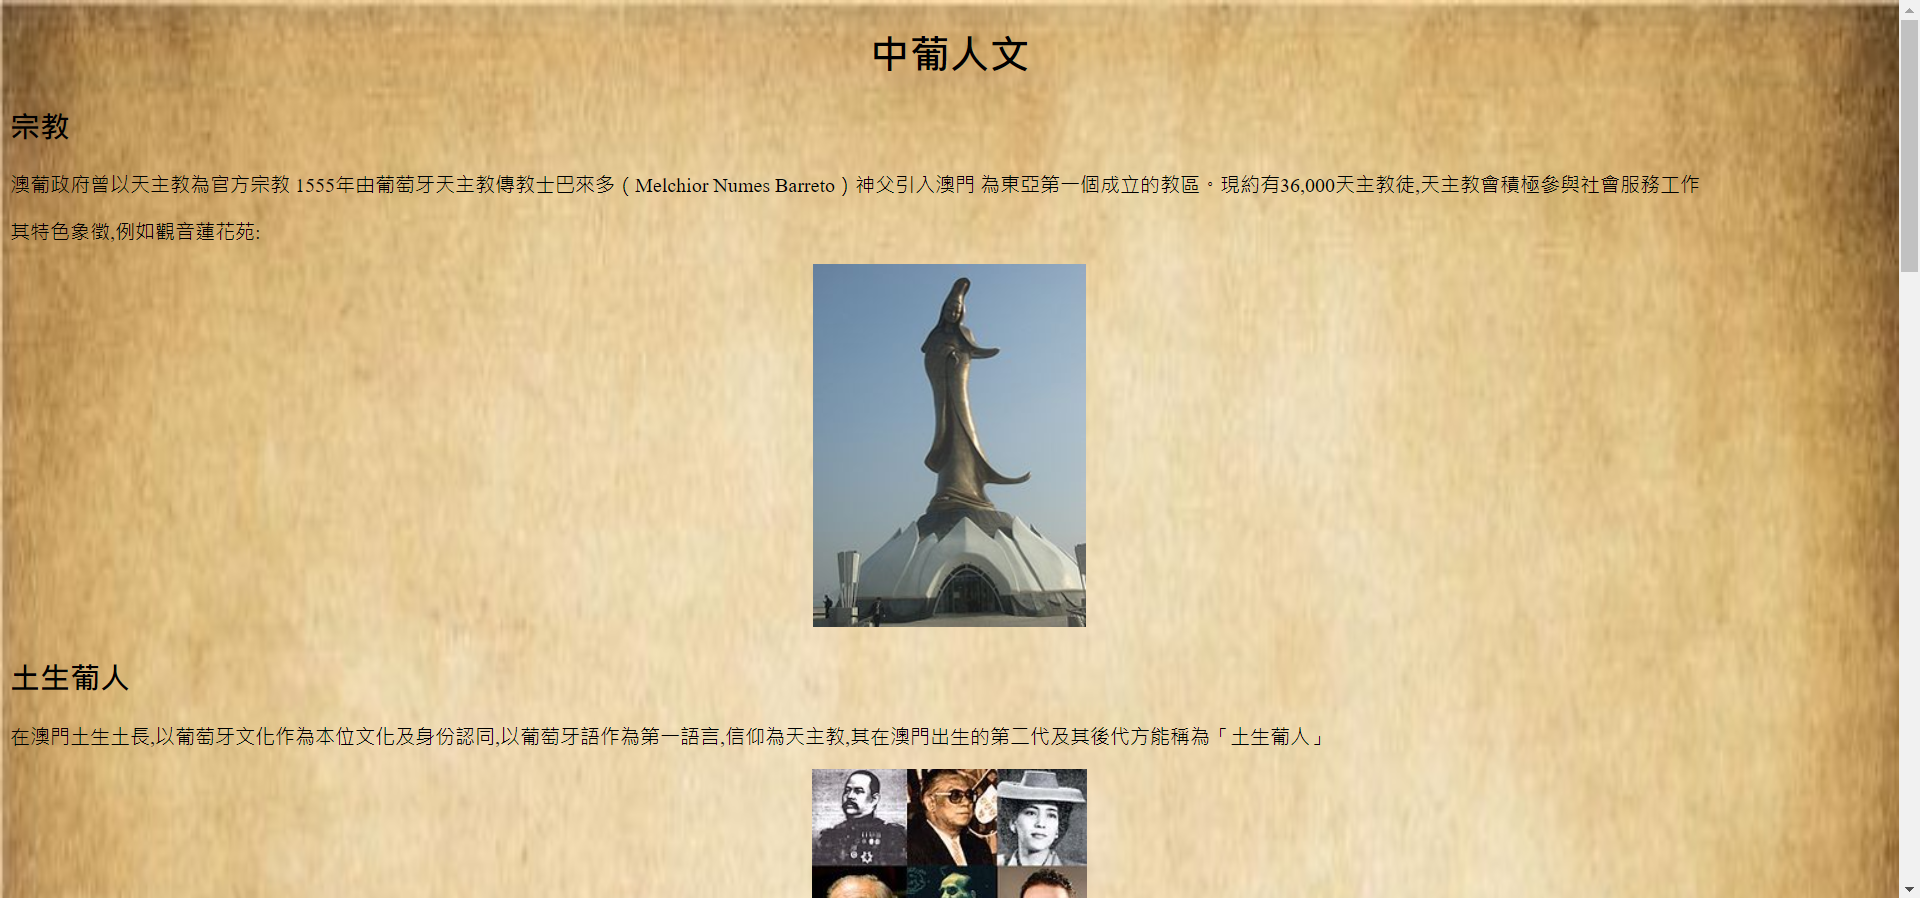
\includegraphics[scale=0.30]{images/3-2.jpg}
			\caption{页面2 (中葡人文)}
			\label{fig3-2}
		\end{center}
	\end{figure}
	\begin{figure}[htb]
		\begin{center}
			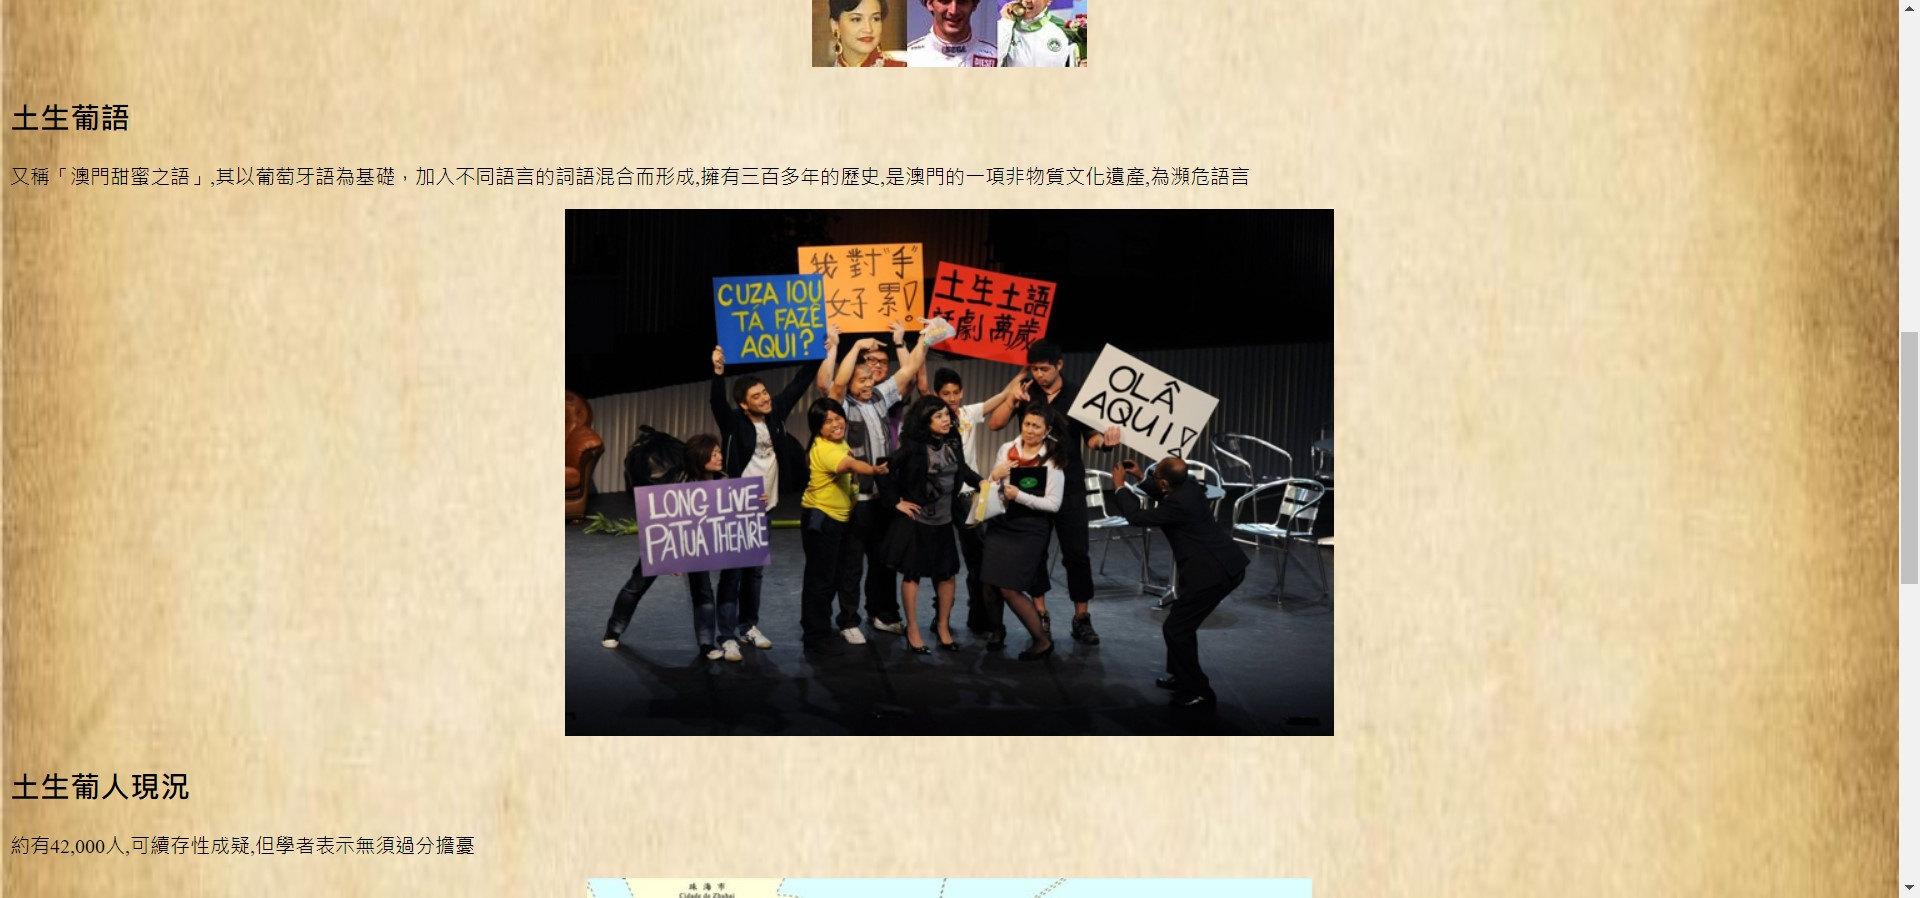
\includegraphics[scale=0.30]{images/3-2-1.jpg}
			\caption{页面2 (中葡人文)}
			\label{fig3-2-1}
		\end{center}
	\end{figure}
	\subsection{页面3 (中葡飲食)}
	这个网页主要介绍了澳门土生葡菜的歷史,典型的土生葡菜烹饪技术和介绍一些獨突的菜色;
	
	首先,我以時間線去描述了土生葡菜的歷史,我使其分为起源和现今兩大部分,著重介绍其出现的原因是源于葡萄牙人把自身文化和風俗与澳门當地華人生活方式结合而成,亦呈现出其现今在澳门當地的主要性;
	
	然后,我更介绍了土生葡菜一些典型的烹饪技术,包括煎、炒、煮、炸、焖、燉、焗、烤、蒸等等,同時亦介绍了其主要的食材、佐料和香料,以及土生葡菜的特色;
	
	最后,我以表格的方式介绍了一些較为著名的土生葡菜,如馬介休、西式臘腸、乾免治、葡国雞、非洲雞以及肥菜等由中、西兩地文化结好而成的土生葡菜,其中加插入圖片,以呈现出這些食物的獨特之處;
	
	以下是网页的部分截图:
	
	
	\begin{figure}[htb]
		\begin{center}
			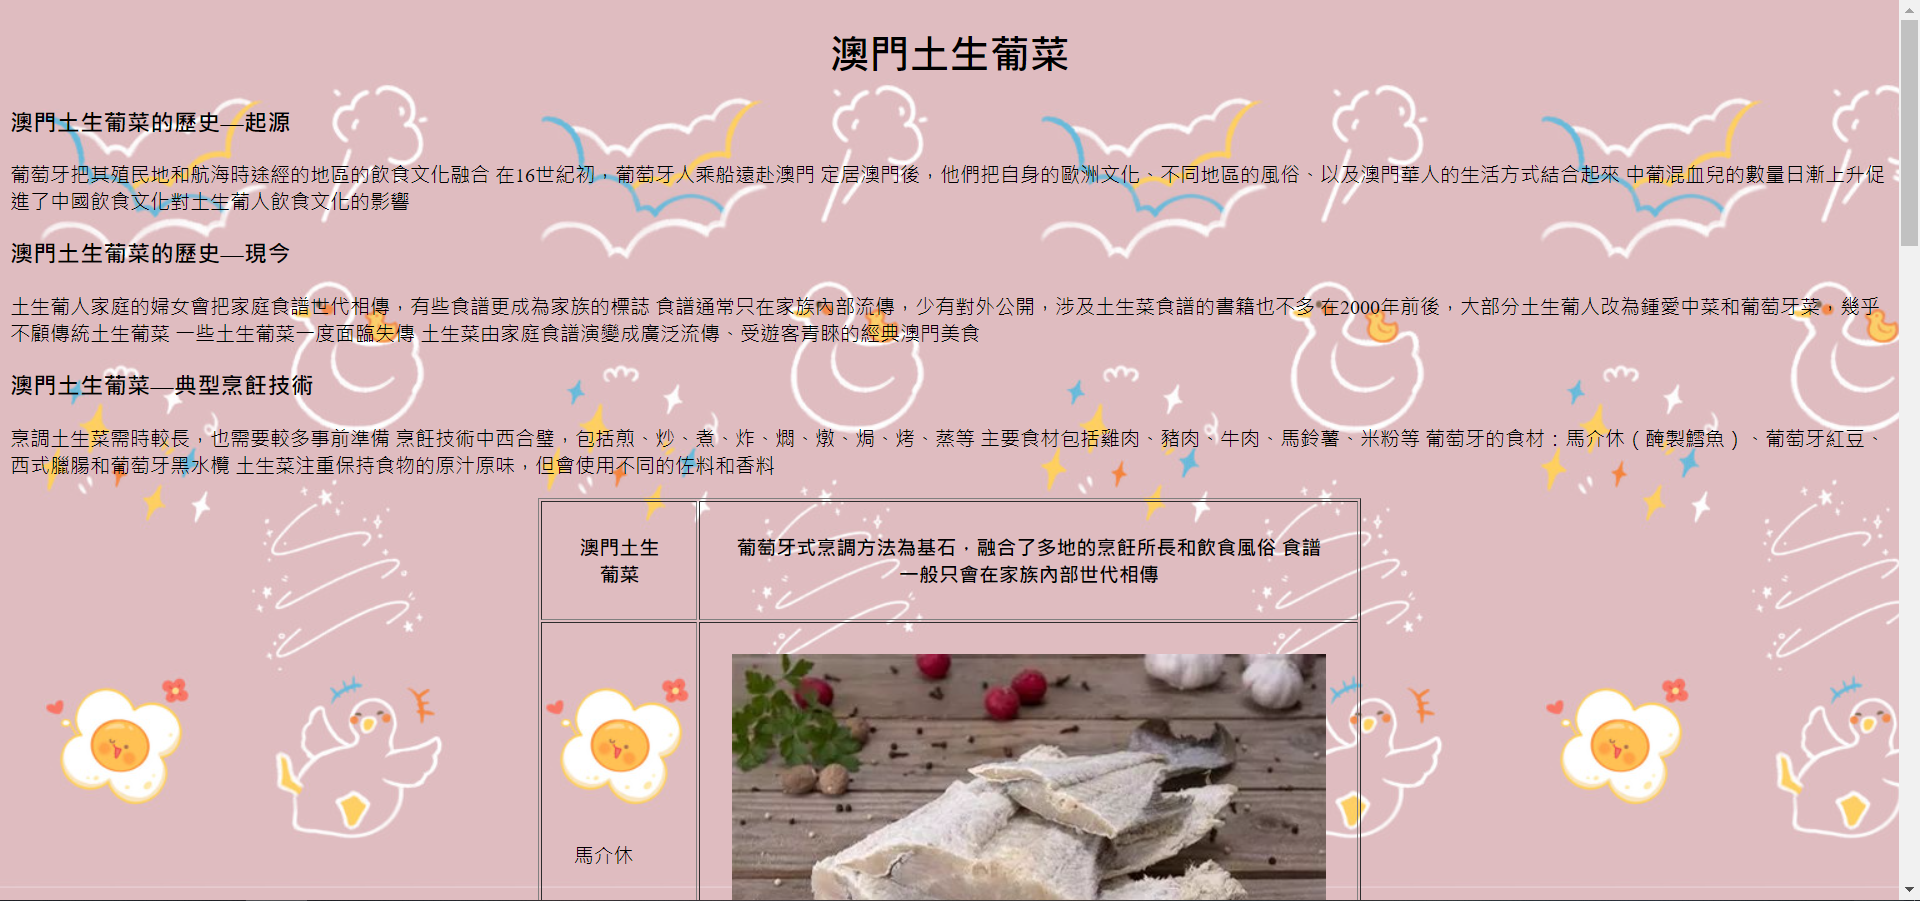
\includegraphics[scale=0.40]{images/3-3.jpg}
			\caption{页面3 (中葡飲食)}
			\label{fig3-3}
		\end{center}
	\end{figure}
	\begin{figure}[htb]
		\begin{center}
			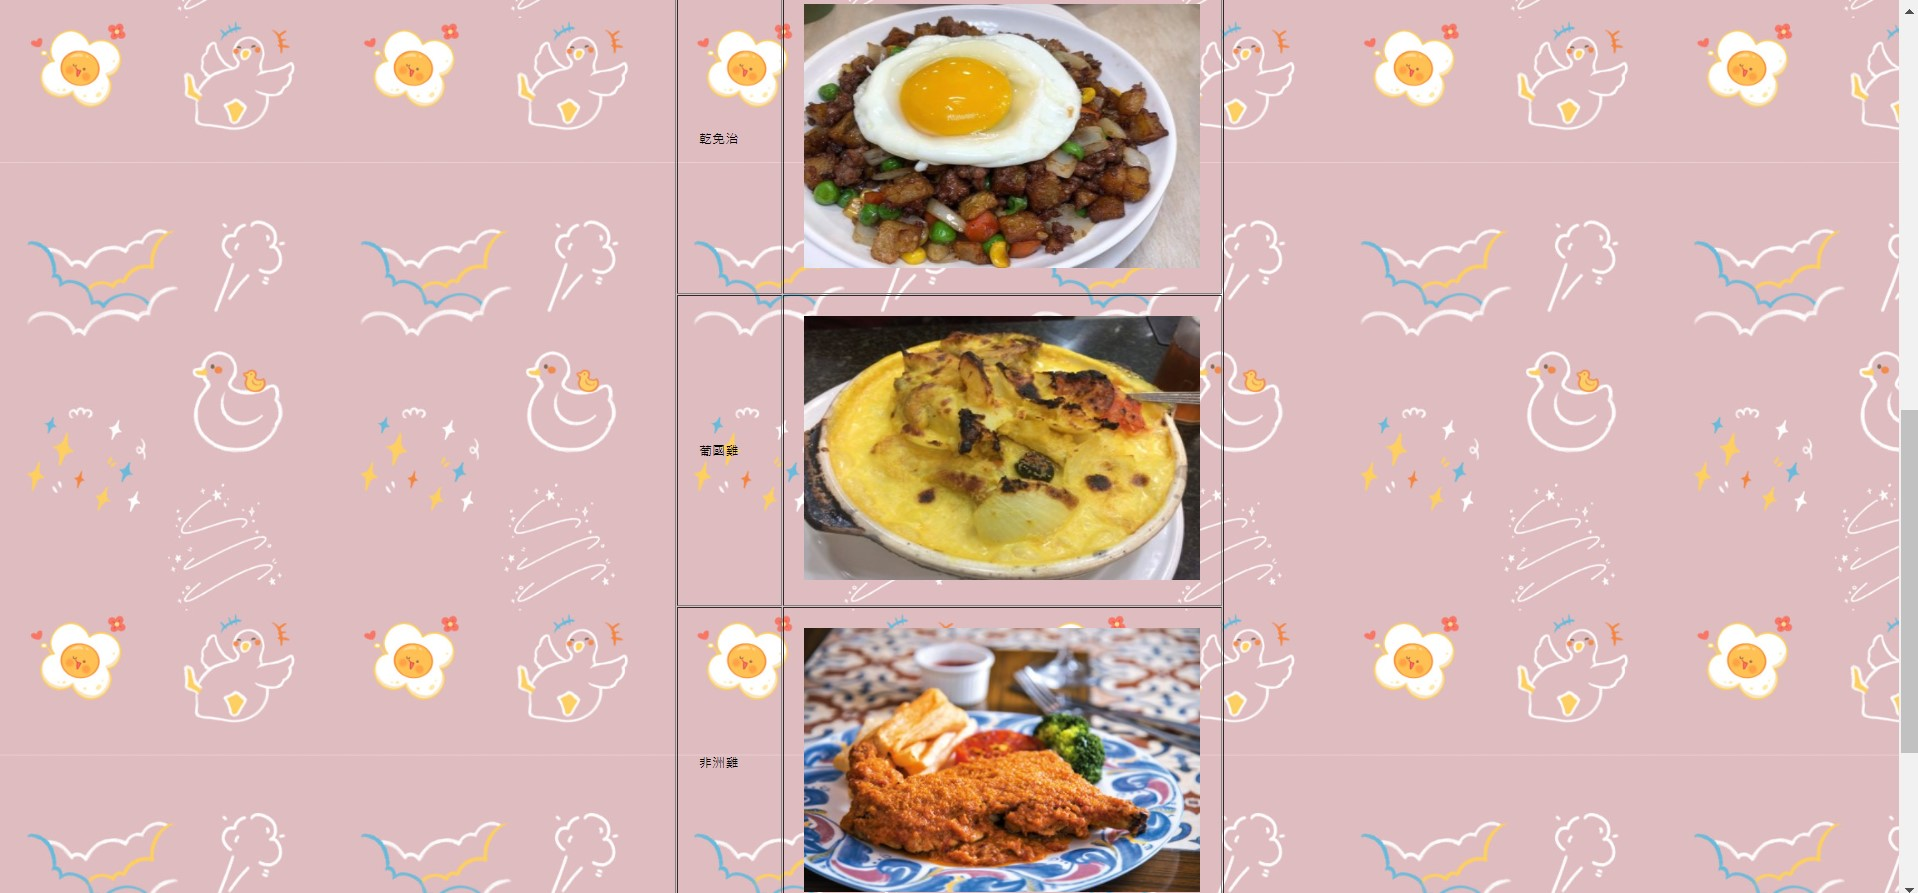
\includegraphics[scale=0.30]{images/3-3-1.jpg}
			\caption{页面3 (中葡飲食)}
			\label{fig3-3-1}
		\end{center}
	\end{figure}
	
	\newpage
	
	\subsection{页面4 (多重国籍)}
	在页面四中,我以兩地不同的法律规定入手,描述了兩个不同国家對多重国籍的规定:
	
	因葡萄牙奉行屬地主义,在其领地出生者即可擁有葡国国籍,而葡萄牙對此多重国籍亦无过多限制;
	
	而中国国籍法的规定則是与其完全相反,其第三條明確规定:中華人民共和国不承认中国公民具有双重国籍。
	
	我更使用兩国的看法表现国为解决這因《中葡聯合声明》而出现的問题,中国更因此进行了兩次人大釋法。
	
	最后,我以表格方式,呈现了澳门中葡混血人士的特殊情况,从供浏览网页者作為參考。
	
	以下是网页截图:
	
	
	\begin{figure}[htb] % here top bottom
		\begin{center}
			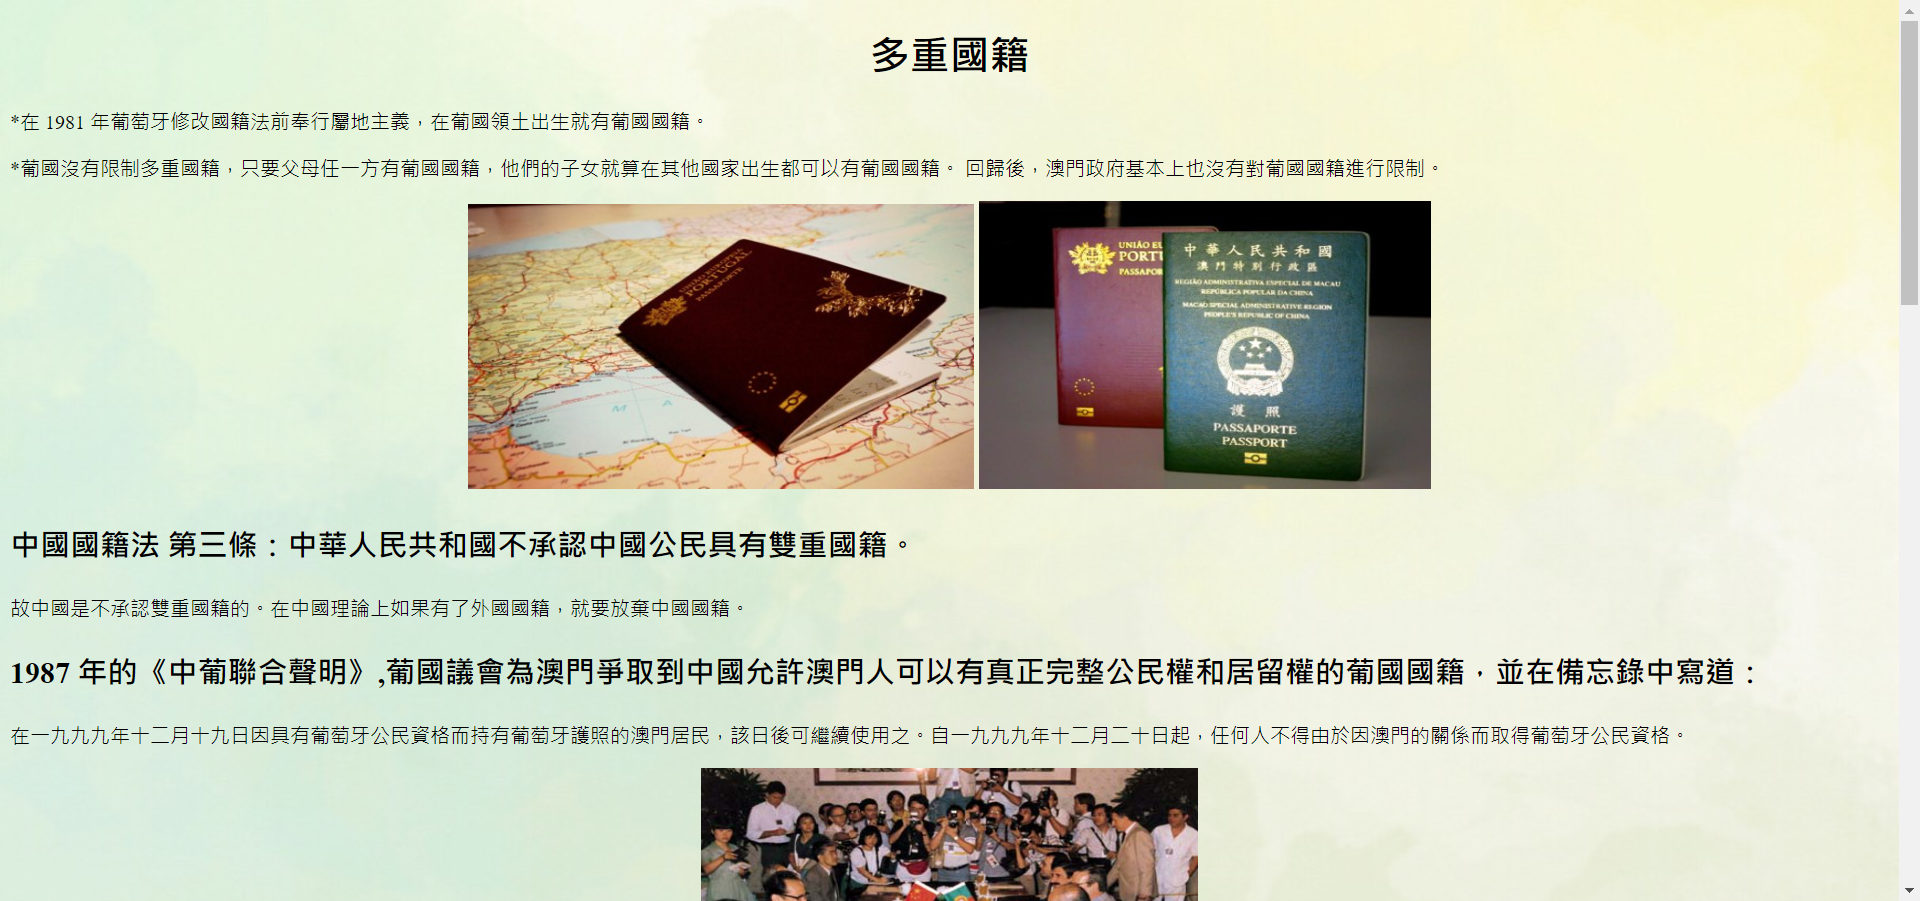
\includegraphics[scale=0.30]{images/3-4.jpg}
			\label{fig3-4}
			\caption{页面4 (多重国籍)}
		\end{center}
	\end{figure}
	
	\newpage
	
	\section{网页设计小结}
	1、缺少思路:
	在设计网页的初期,我没有準確的方向,不知道如何尋找出一个正確的思路去设计出一个自己的网页。我想做出一个能令人满意的网页,但我卻被自身的技术不足所限制,没有足夠的技术,很多想法都難以實施,故最后更是寸步难行;在此之後,我便萌生了随随便便做个网页,把作业交了就可以了,但看到身边的同学、室友們都認真地把网页完成,我那开混的想法又开始有所动摇,因此我纠结了很久。最后在纠结數天後,在与室友的溝通中,我特然發现国內的同学对澳门的了解和認知都不是很清楚,在發现此問题後,我最终决定做了一个介绍关于我的家乡澳门所特有的“中葡文化”的网页,用以和同学分享這座小城的獨特文化。
	
	2、技术不成熟:
	课堂上時間有限,不可能在短短的四小時內把网页設計這一个庞大的主题全部教给我们,而老师更不可能幚助我們解决所有问题,這导致我難以去把我所有的想法转变为實際內容。对于这个问题,我只能透过一次次地询问同学、室友等,和他们讨论,寻求問题的解决办法;第二个就是上网查找,网上的內容極为豐富,其中必定存在与我想法一致的人,透过查询网上的資料和资源模板等,我便能找出一些可使用的代码,以供作參考;
	
	比如:让图片铺满背景:
	
	\begin{shaded*}\begin{alg}{一个复杂算法}
			\begin{algorithmic}
				\ background-size:100$\%$100$\%$
			\end{algorithmic}
	\end{alg}\end{shaded*}
	
	总结:在学习过程中,我們在教师的帮助下,在课室中紧紧围绕一个共同的任务活动中心,通过学习资源的积极主动应用,进行自主探索和互动协作的学习。
	
	然而,老師在課堂上的時間有限,不能完全地講述每一處设计网页的小细节,设计网页入門難度不高,一张图片又或是一篇文章即可完成,但精通于网页设计這项技术卻並不简单,很多好的想法卻因技术不足導致難以實现。
	
	而我为解决此問题,浏览了一些比较熟悉的网页,透过找出该网页吸引我的优点,了解网页设计中关于色彩搭配和布局的知识,有效地提过了自己的水平,如文本,图像,表格,链接,CSS样式等不同区块的應用,我都有所掌握,而水平亦有所提高。
	
	我更采用了模仿式的学习手法,着重学习不同网站的整体效果设计与制作,通过学习模仿优秀网站的设计,提高了自身的审美能力,对各类网站的设计风格,色彩搭配,网页布局等有一定的认知。
	
	感谢此次的网页设计課,此不僅学会了一門重要技术,同時各方面都有所提升,通过不同的学习方法,解决自身問题,而這些经历都是绝无仅有的。
	\newpage
	
	\section{课程的收获和建议}
	
	\subsection{计算机基础知识}
	以下为我在課堂中所学习到的知识,我將列点説明:
	
	1、计算机的广泛应用,在自然语言,语音技术,图像技术,视频技术,知识图谱,数据智能,增强学习,深度学习等方面都有着重要的作用。
	
	2、我国在超级计算机行业领先世界。比如中国在1983年就研制出第一台超级计算机银河一号, 使中国成为继美国、日本之后第三个能独立设计和研制超级计算机的国家,2011年中国拥有世界最快的500个超级计算机中的74个,中国以国产微处理器为基础制造出本国第一台超级计算机名为“神威蓝光”;又比如神威·太湖之光超级计算机是由国家并行计算机工程技术研究中心研制、安装在国家超级计算无锡中心的超级计算机, 上面安装了40960个中国自主研发的“申威26010 ”众核处理器, 该众核处理器采用64位自主申威指令系统, 峰值性能为12.5亿亿次每秒, 持续性能为9.3亿亿次每秒。2017年11月13日, 全球超级计算机500强榜单公布, “神威·太湖之光”以每秒9.3亿亿次的浮点运算速度第四次夺冠。2018年11月12日, 新一期全球超级计算机500强榜单在美国达拉斯发布, 中国超算“神威·太湖之光”位列第三名。这些事情使我自豪。
	
	3、知道了面临的技术和安全挑战如制造工艺落后,美国对5G的打压。
	
	4、了解了计算机的发展,如知道了一个抽象的机器图灵机,世界第一台电子计算机ENIAC,知道了计算机发展的特点体积越来越小, 可靠性越来越高,电路规模越来越大, 速度越来越快,功能越来越强大;知道了未来计算机的发展方向:微型化、巨型化、网络化、智能化。
	
	5、知道了计算机的系统组成分为计算机软件系统和计算机及硬件系统,知道了计算机的主板组成分为PCI插槽,AGP插槽,CPU插槽,(主存)内存插槽,硬盘IDE插槽,,软盘IDE插槽,ROM,南桥芯片组,北桥芯片组,USB,接口组,游戏、声音接口组,并行、串行接口组,电池。
	
	6、知道了影响CPU运行速度的因素:主频,核心数,Cache, 高速缓存,寄存器,流水线,字长,指令集等;
	
	这个专题在讲述时非常具体详细,但是總体而言卻令我感到与課堂无关,後半節課堂为打字練习,但卻没有實際的要求,令我不能感到此課堂的作用。	
	\newpage
	\subsection{文档撰写工具LaTeX}
	
	1、学习latex时我学会了很多latex不同的功能,如章节自动编号$\backslash$section,又如文献、图表自动引用$\backslash$cite和$\backslash$ref。
	
	2、我更知道了从源文件.tex的第一行命令$\backslash$documentclass开始,至命令$\backslash$begin$\left\{document\right\}$语句统称为导言,$\backslash$begin$\left\{document\right\}$与$\backslash$end$\left\{document\right\}$之间的所有命令称为正文,$\backslash$end$\left\{document\right\}$之后的任何字符, LaTex都会忽略。
	
	3、我学会了自定义新命令$\backslash$newcommand$\left\{\right\}$参数数量,默认值$\left\{\right\}$。
	
	4、同時学会了宏包的调用$\backslash$usepackage。
	
	5、知道bib文件这一个东西,即用LaTeX写文档时, 一般用.bib文件来管理参考文献, 这种方式能自动在引用的时候定义参考文件的序号, 不需要人工进行编号,十分方便。
	
	6、学会了如何去引用,比如引用页码$\backslash$pageref$\left\{\right\}$。
	
	总结 LATEX 的一些优点:具有专业的排版输出能力,产生的文档看上去就像印刷品一样;具有方便而强大的数学公式排版能力,无出其右者;而绝大多数时候,用户只需专注于一些组织文档结构的基础命令,无需操心文档的版面设计;同時latex很容易生成复杂的专业排版元素,如脚注、交叉引用、参考文献、目录等,latex亦具有强大的可扩展性。然而缺点也是显而易见的:入门门槛高。
	
	建议:因为其入门门槛高,我認为一节课堂並不足以讓我們有效地完全掌握其主要核心内容,故我認为可为其增加一節,讓学生有效地学习到這项门槛高但極为實用的工具。
	\newpage
	\subsection{编程工具Python}
	
	1、对python有了最基本的了解:Python由荷兰人吉多ꞏ范ꞏ罗苏姆于1989年编写的一个脚本解释程序,语法优雅,可读性强;Python可运行在多种计算机平台和操作系统中, 如unix、windows、Mac OS、Ubuntu、OS/2等等;Python语言具有简洁性、易读性以及可扩展性,应用广泛。并且知道了python的应用场合如人工智能,云计算,大数据,网络爬虫,自动化运维,web开发,科学计算,常规软件开发。
	
	2、知道如何在Windows系统中安装Python:进入Python官方网站www.Python.org下载安装包进入Windows版的下载页面,下载Windows x86-64 executable installer或者Windows x86-64 executable installer,之后同时按键盘上的窗口键和r键, win+r输入cmd按确认或直接回车,输入“Python”或“python” 。之后安装开发环境安装pycharm与anaconda:win+s 搜索prompt (或在安装路径) 打开Anaconda Prompt, 配anaconda环境或者在开始菜单查找Anaconda Prompt,在anaconda命令行中, 敲入: conda create -n 自选路径名字如DL python=3.7, 选择anaconda环境安装路径。在anaconda命令行中, 敲入: conda activateDL, 激活开发环境,并配置开发环境:输入conda create -n dl python=3.7,然后装python, 敲y回车,这之后敲conda activate dl, 回车, 激活环境。安装opencv:敲入conda install -c menpo opencv。
	
	3、知道了python一个重要的特点在Python的代码块中必须使用相同数目的行首缩进空格数。
	
	4、输入函数input,输出函数print。
	
	5、学习了数据转换,函数的调用,矩阵的运算,循环的控制。
	
	总结而言Python具以下优点:
	1.简单容易学习,Python是一种代表简单主义思想的编程语言。阅读一个良好的Python程序就像读英语一样。它使你可以更专注的去解决问题而不是去搞清楚问题语言本身。2.速度快:Python的底层使用c语言写的,很多标准库和第三方库也都是用c语言写的,运行速度也非常的快。
	3.可拓展性:如果需要一段关键代码运行得更快或者希望某些算法不公开,可以部分程序用c或者c++编写,然后在Python程序中使用他们。
	4.丰富的库:Python标准库确实很庞大。它可以帮助处理各种工作。而除了标准库以外,还有许多其他高质量的库,如wxPython,twisted和Python图像库等
	简单来说,Python就是简单易学,功能强大的编程语言。
	建议:此项共有两节课堂,能令我有效地理解python,然而,一門語言的学习绝不是輕易就能成功的,雖然老師所编写的代码的幫助下我能理解部分內容,然而在當時没有c语言的基础下,不能很好地理解如數组、包等概念,故希望此課堂放在後一点,在学生擁有一些c的基础下,再教python這門語言,我相信学生在有基础下学习會更为简单。
	\newpage
	\subsection{图像设计软件Photoshop}
	
	1、了解了Visio的使用,即Visio一款便于IT和商务人员就复杂信息、系统和流程进行可视化处理、分析和交流的软件,正是因为会使用他,实验报告中的网页整体框架我才能轻松的设计出来。
	
	2、会使用历史记录画笔,即可以将已经改成黑白的照片还原回来,具体操作为:选择历史记录画笔, 设置笔触, 用笔触涂抹将人勾画出来。
	
	3、会使用:仿制图章工具,即可以准确复制图像的一部分或者全部, 从而产生某部分或者全部的拷贝, 是修补图像时常用的工具,具体操作为:按住ALT在图像某一处单击。
	
	4、学会建立选区及学会使用选取工具。
	
	5、学会用魔棒做透明签名:用菜单图像——调整阈值——128——确定实现去色, 转化为二值图效果,用魔棒选中白色区域, 按delete键删除背景,之后保存为png格式文件。
	
	6、还学会了斜切,拉长腿和换脸技术。
	
	總体來説PS可以用于平面设计、广告摄影、影像创意、网页制作、后期修饰、视觉创意、界面设计等。其具有应用性广、技术性强等优点。PS同時具有优良可塑性,由此可见PS是一个極为實用的功具。
	\newpage
	\subsection{版本管理软件Git}
	
	这节课总体来说学习了一下知识Fetch/clone:更新/克隆一个远程仓库到本地,Push:推送本地仓库到远程仓库,Pull:从远程仓库更新本地文件,Checkout:从本地仓库更新文件,Add:添加本地文件到暂存区,Commit:提交本地修改到本地仓库。
	
	1、clone:git clone https://gitee.com/chenjz70/experimental-report。
	
	2、push:  git push -u origin master。
	
	3、pull:  git pull origin.
	
	4、add:   git add .
	
	gitee的优点:项目集中管理,更利于管理,缺点:无法精确到针对某一项目协作管理。
	我在使用gitee时遇到了一些困难,因其部分功能需要进行實名認証方可使用,而卻无提出港澳台的實名方法,故一些服务我无法使用,希望課堂能使用港澳台学生也能使用的工具,以助我們能顺利学习。
	\newpage
	
	\subsection{网页制作Dreamweaver}
	
	1、设置页面属性:在出现的“页面属性”对话框中进行相应设置。
	
	2、插入图像image:单击选择“插入”菜单下的“图像”命令, 弹出“选择图像源文件”对话框。
	
	3、在主页中建立超链接:在出现的图片上右击, 从快捷菜单中选择“属性”命令, 在图片下方将出现“属性”对话框,在“属性”对话框中单击“矩形热点工具”并选定区域,在该热点上右击出现的“属性”对话框中进行属性设置,设置链接、目标与替换。
	
	4、建立新闻页面:文件——新建——新建文档——文档类型HTML——框架——无——创建,单击选择“文件”菜单下的“另存为”命令, 弹出“另存为”对话框,并保存到相应的路径。
	
	5、设置外观颜色:“文件 “页面属性”命令, 在出现的“页面属性”对话框中进行相应设置: 单击“分类”列表框中的“外观(CSS)”选项, “背景颜色”和“文本颜色”分别设置为对应的颜色。
	
	6、插入表格:单击“插入”菜单下的“表格”命令。
	
	7、把表格隐藏:将边框粗细调整为0。
	
	8、增加外部链接:选中相应部分,并点右边面板上的hyperlink。
	
	Dreamweaver优点如下:
	1.制作效率:Dreamweaver可以用最快速的方式将档案移至网页上。
	2.网站管理:使用网站地图可以快速制作网站雏形、设计、更新和重组网页。
	3.控制能力:Dreamweaver是唯一提供Roundtrip HTML、视觉化编辑与原始码编辑同步的设计工具。
	Dreamweaver的代码提示很强大,有设计模式,直接点击,不用敲代码。故我認为它很適合网页设计新手。
	
	\nocite{*} %% 作用是不对文献进行引用,但可以生成文献列表
	
	%\bibliographystyle{HustGraduPaper}
	%\bibliography{HustGraduPaper}
	
\end{document}
